\clearpage
\chapter{Diagramme}
\section{UML-Diagramme}
\subsection{Idee/Erstes UML-Diagramm}
Das Erste UML-Diagramm entstand nach dem ersten Brainstorming in der Analysephase. Alle Teammitglieder diskutierten über das mögliche Spielkonzept. Dabei wurden die ersten Ideen gesammelt und aufgrund der Ideen wurde das erste UML-Diagramm entwickelt. \\
Nach weiteren Besprechungen und zu Beginn der Umsetzung des UML-Diagramms, traten verschiedene Fehler auf, aufgrund eine Implementierung zu diesem Zeitpunkt unmöglich war. 
Beispielsweise wurde die einzelnen Uhren nicht im jeweiligen Unternehmen erzeugt, d.h. der Spieler hätte keinen Zugriff darauf oder, dass ein Spielbrett zur Verwaltung des kompletten Spielablaufs gefehlt hat.

\begin{figure} [h]
	\centering
	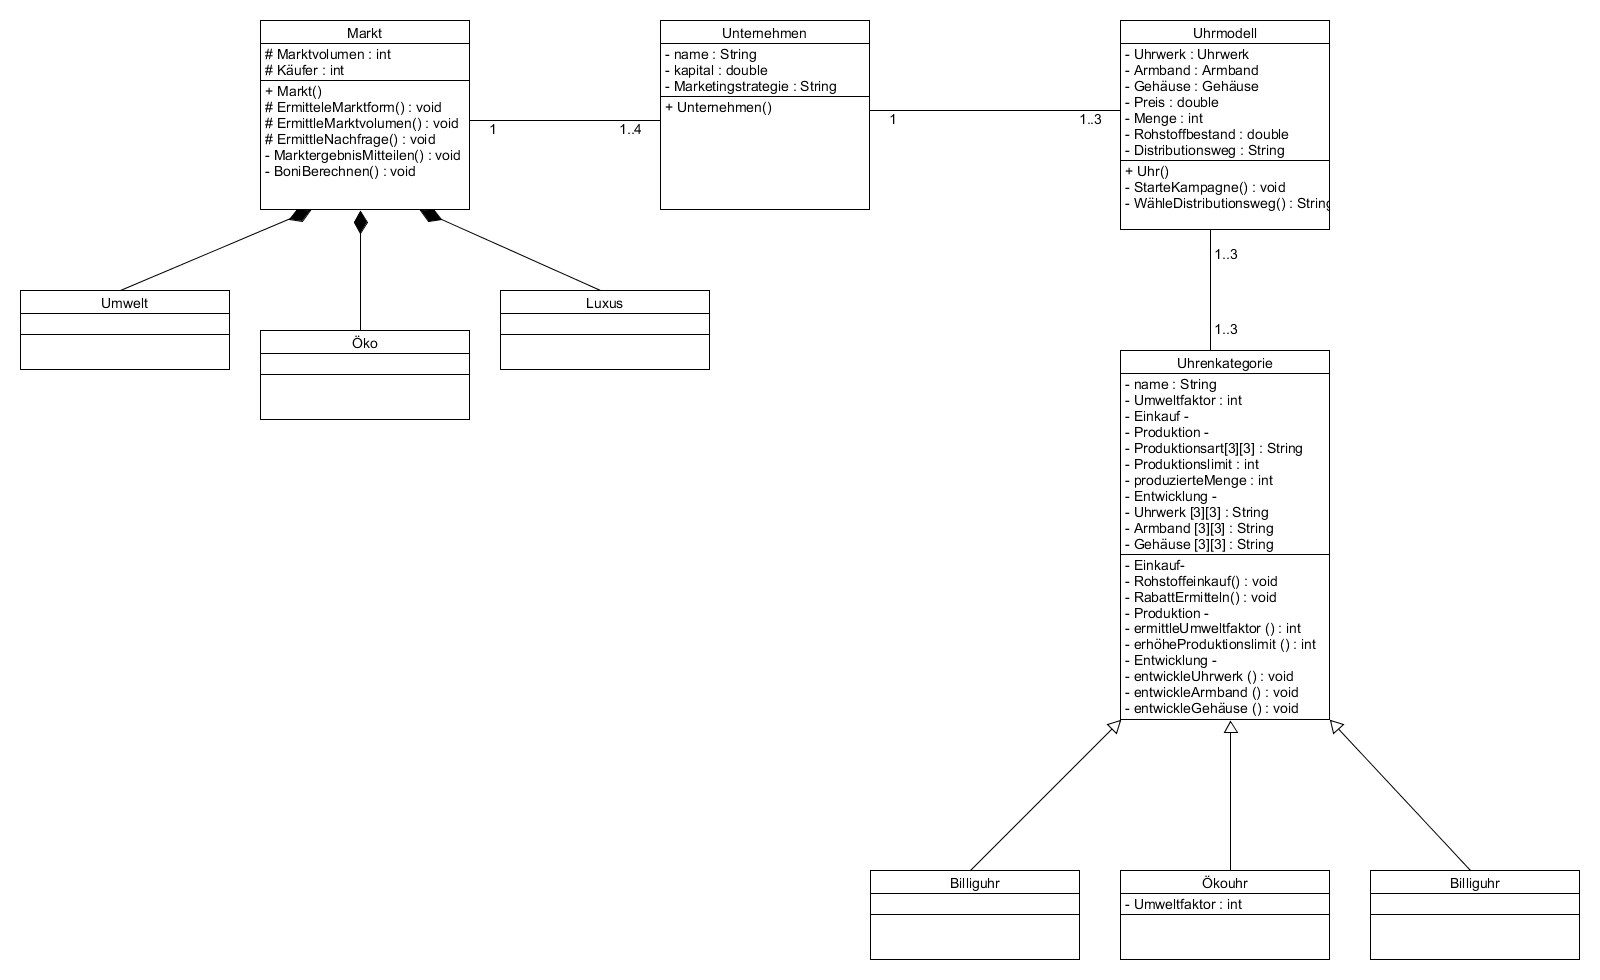
\includegraphics[scale=0.35, angle=90]{img/ErsterEntwurfUML.png} 
	\caption{Erstes UML} \label{fig:abb26}
\end{figure}

\clearpage
\subsection{Finales UML/Unternehmenssimulation}
Das Finale UML-Diagramm der Unternehmenssimmulation entstand bei der Erstellung des Fachkonzeptes. Während der Entwicklung des Diagrammes wurden mehrere Meetings gehalten, das UML-Diagramm verbessert und die Entwürfe ins Fachkonzept umgesetzt. Die anstehenden Fehler wurden wiederum im nächsten Meeting besprochen und das Diagramm angepasst. Am Ende der Entwicklungsphase war das Finale UML-Diagramm fertig.
\begin{figure} [!h]
	\centering
	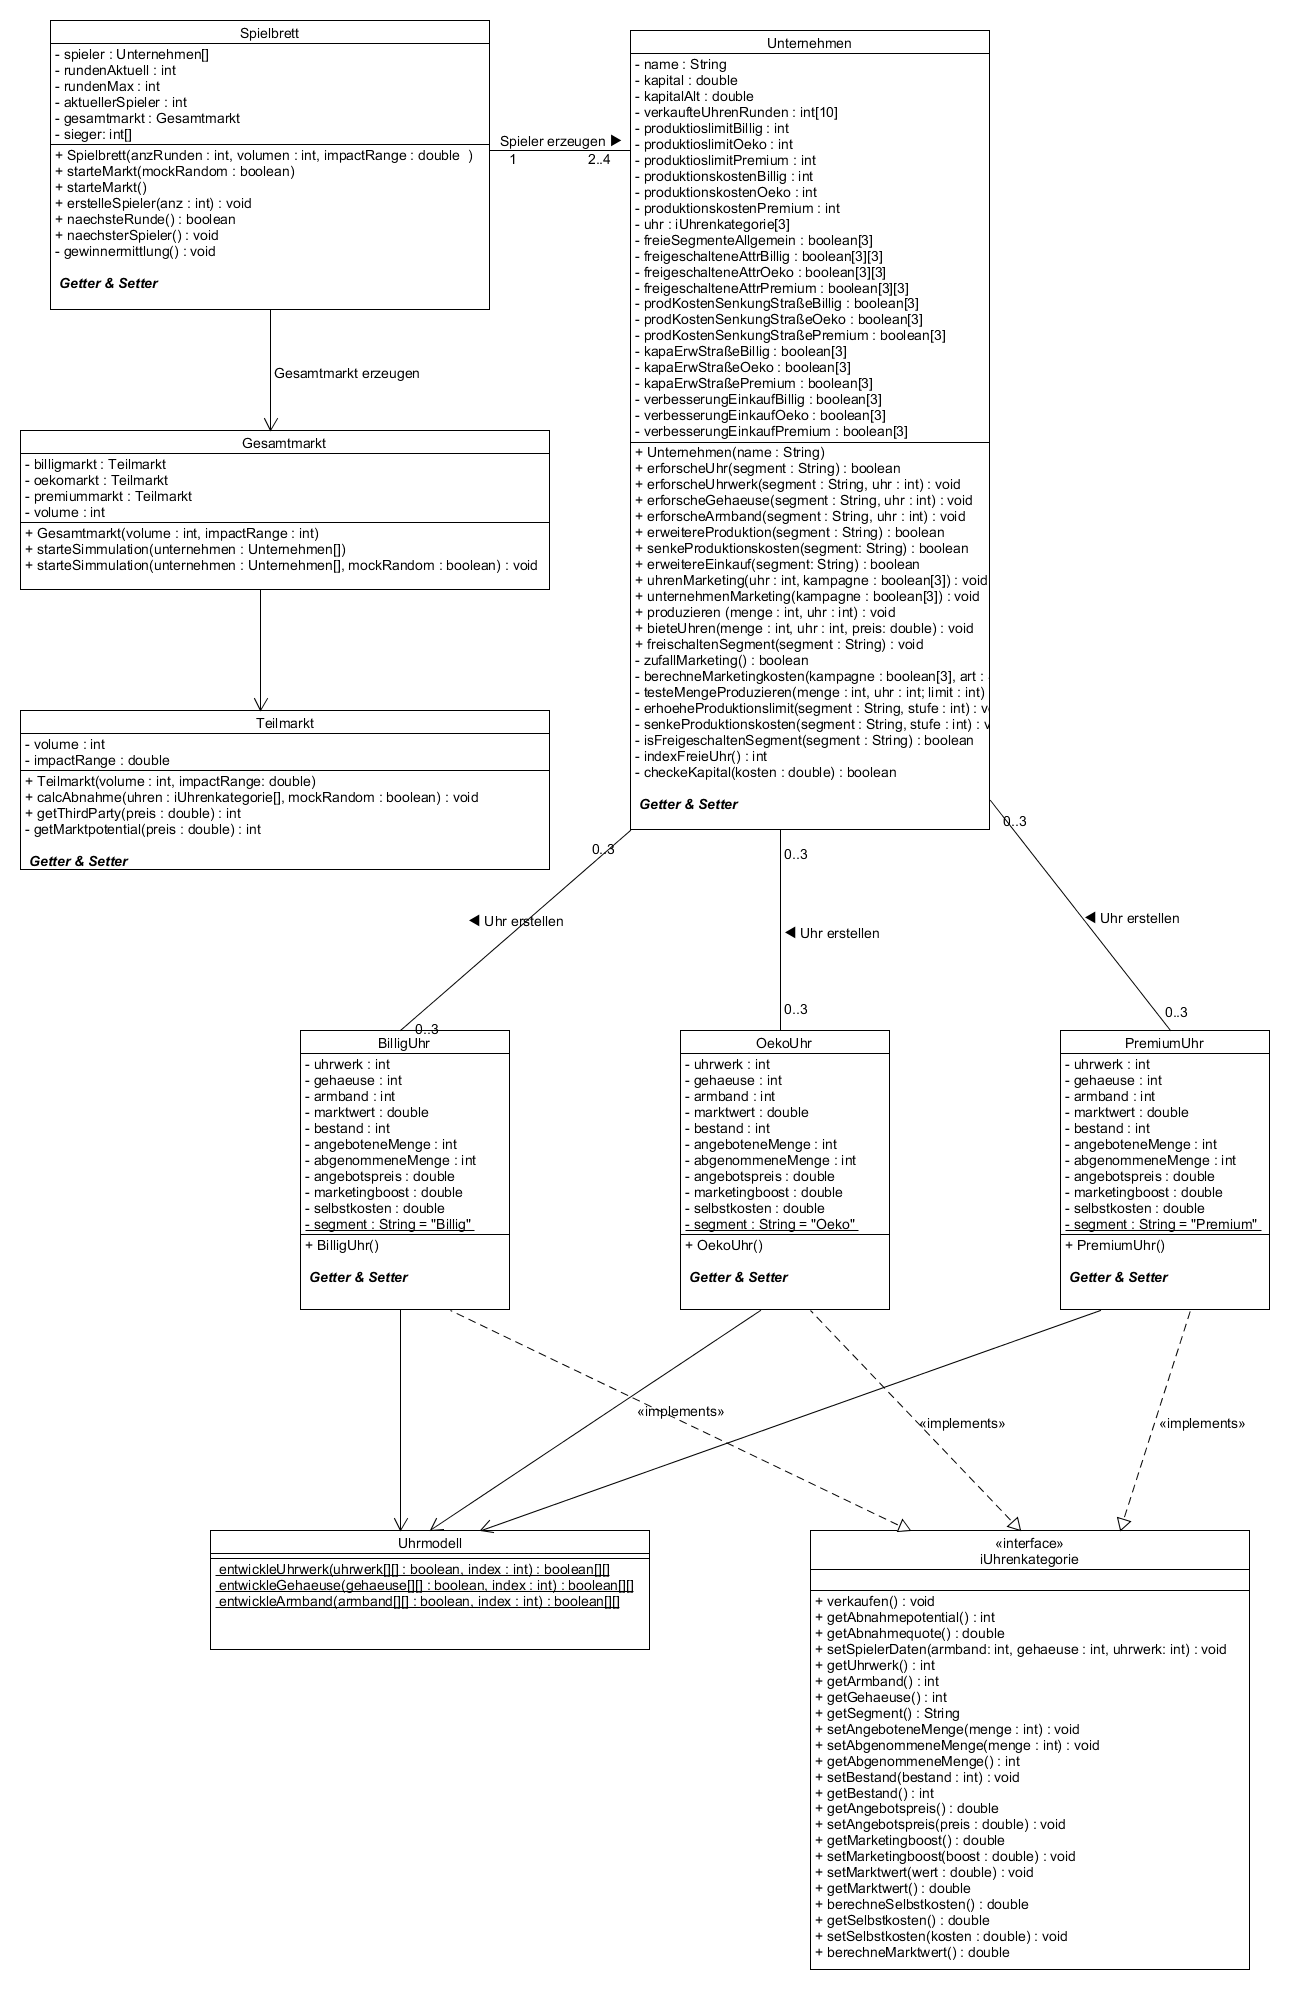
\includegraphics[scale=0.3]{img/Unternehmenssimmulation_final.png} 
	\caption{Finales UML von \enquote{Watch Tycoon 2017}} \label{fig:abb27}
\end{figure}

\clearpage
\section{Zustandsdiagramm}
\begin{figure} [!h]
	\centering
	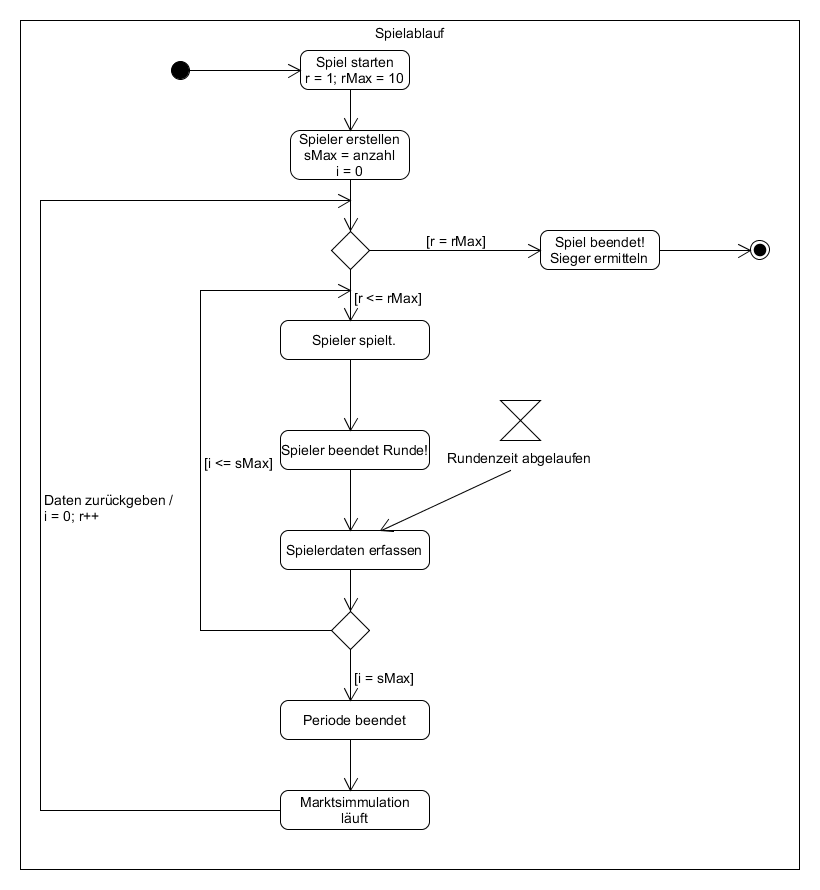
\includegraphics[scale=0.5]{img/Spielablauf.png} 
	\caption{Zustandsdiagramm einer Spielrunde} \label{fig:abb28}
\end{figure}





